\section{Results and Analysis}
For each experiment five algorithms are studied.
A basic implementation of $A^*$ that serves as reference,
the three proposed variations $A^*mbush$, $P$-$A^*mbush$
and $SAR$-$A^*mbush$ and finally a Randomized Spanning Tree $RST$.
The last one is an algorithm that generates random trees that
cover all the  graph. It can be interpreted as a change in
the agent's cost function by assigning the value of infinite
to several edges in the map. The  $RST$ is different for
each agent, with the goal of generating paths that are
variate and stochastic.

For the experiments, two different map instances were 
considered as they are and as a base for bigger maps. 
The first one (see Figure \ref{fig:gs}) is composed
by 60 polygons, the second one (see Figure \ref{fig:gs}), has 85.
All the polygons are convex, in order to reduce the verification costs
when checking which polygon a point belongs to \cite{web1}. 
Each node in the graph is induced by a polygon in the map, 
located in it's geometric centroid \cite{book3}.

The cost function is common to all agents. The cost is proportional
to the euclidean distance between the polygon's centers. 

\begin{figure}[htb]
	\centerline{
		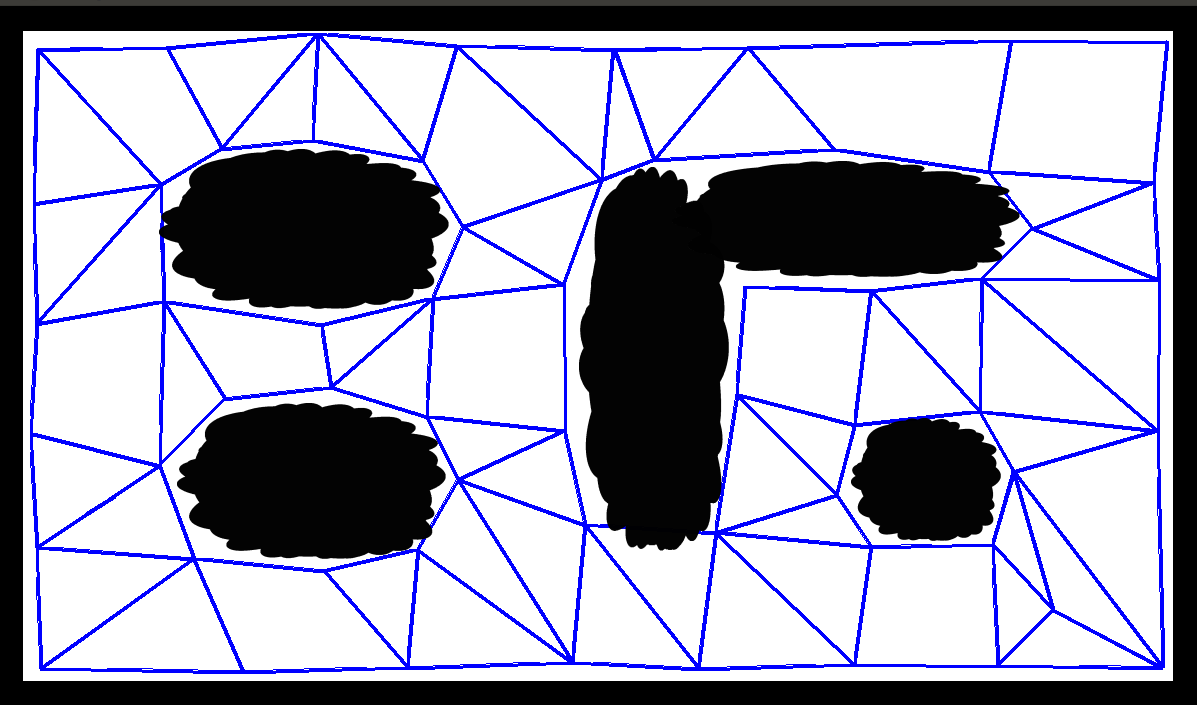
\includegraphics[width=0.48\columnwidth]{figures/g2.png}
		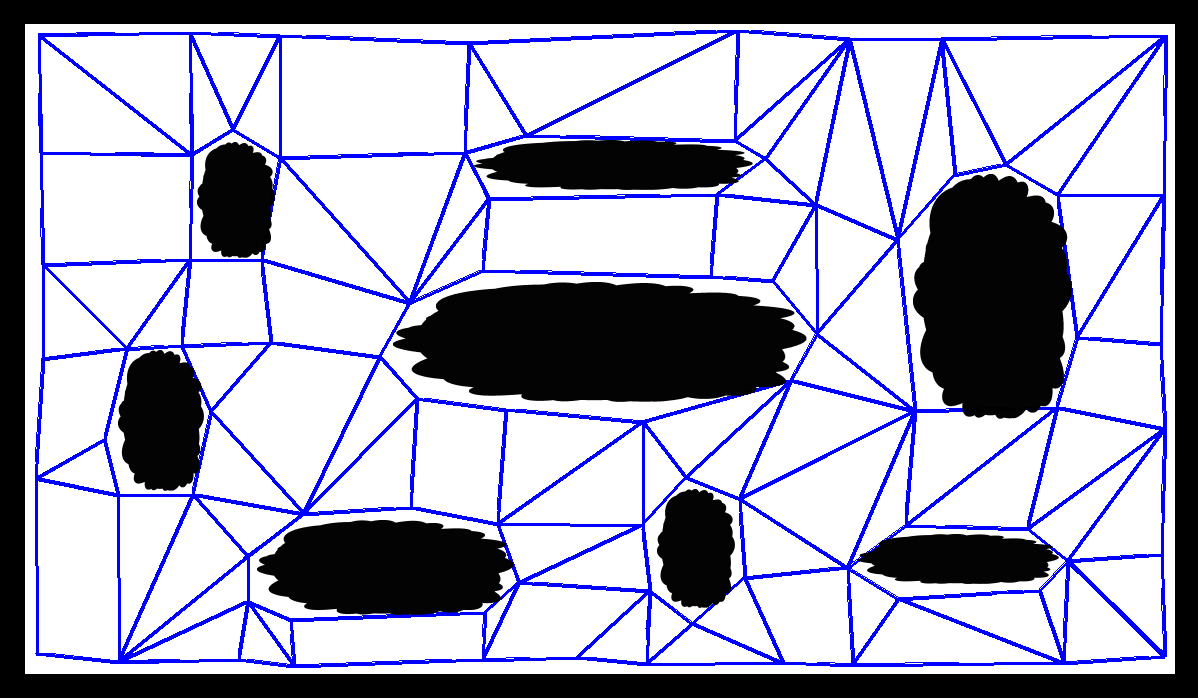
\includegraphics[width=0.48\columnwidth]{figures/g1.png}
	}
	\caption{\label{fig:gs}
	     Left: Polygonized map 1 (60 polygons).
	     Right: Polygonized map 2 (85 polygons).}
\end{figure}

Experiments with variable agent numbers were performed.
The results are described in section \ref{sec:Globals}. 

The ambush degree ($\Phi$) towards the goal node is shown for the 
following algorithms: $A^*$, $RST$, $A^*mbush$, $P$-$A^*mbush$ 
using real ($A^*$) distance and $SAR$-$A^*mbush$.
Besides the ambush degree ($\Phi$), the incremental cost mean is 
shown. This measure displays the mean of  the percentage's increment
in the cost of the paths generated by $RST$, $A^*mbush$,
$P$-$A^*mbush$ and $SAR$-$A^*mbush$ when compared to the minimal
costs obtained with $A^*$.

\begin{comment}
\subsection{Experiments with three agents}.

 Figure \ref{fig:ambush1} shows the behavior for $A^*$, $RST$, $A^*mbush$
  and $P$-$A^*mbush$ in map 2. The agents are represented by small 
  circles and the goal is symbolized by a red cross.
  
  All the paths are shown raw, namely, the displayed routes
  are the direct joints between the polygon's centroids. This
  generate rough movements. Nevertheless, path smoothing
  algorithms can be used \cite{book3} to avoid sharp changes
  in the orientation of the agents.
  
  
  \begin{figure}[htb]
	\centerline{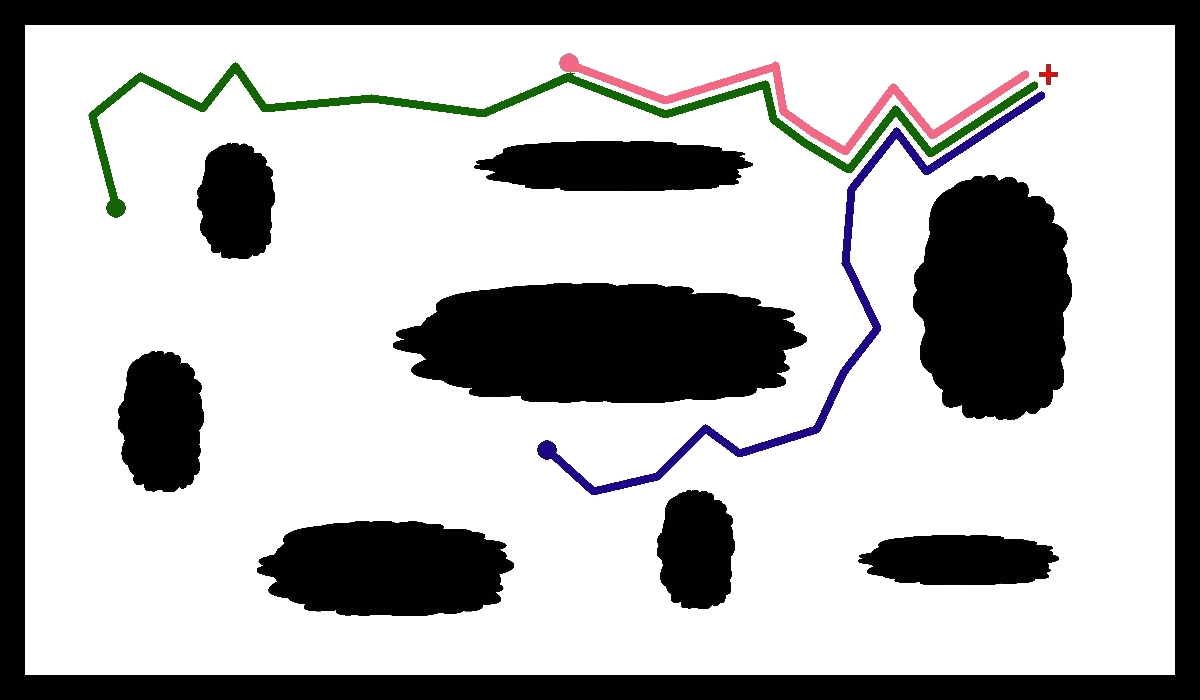
\includegraphics[width=0.7\columnwidth]{figures/instance/Astar.jpg}}
	
	\vspace{0.15cm}
	\centerline{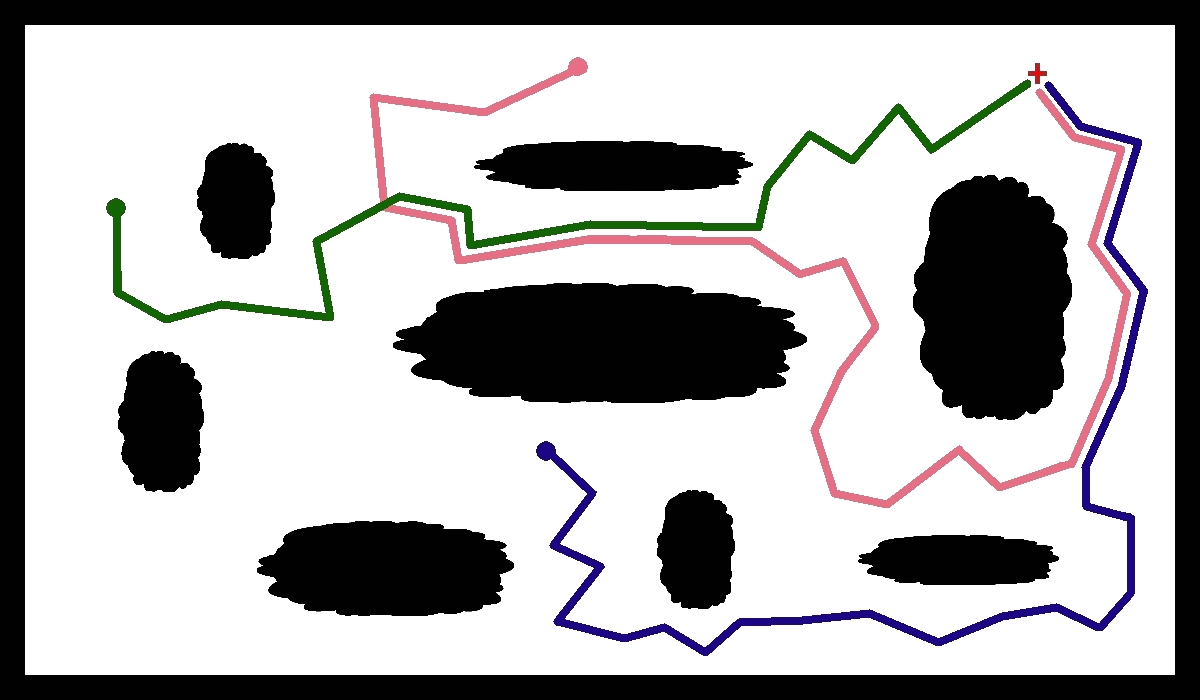
\includegraphics[width=0.7\columnwidth]{figures/instance/RST.jpg}}
    
    \vspace{0.15cm}
	\centerline{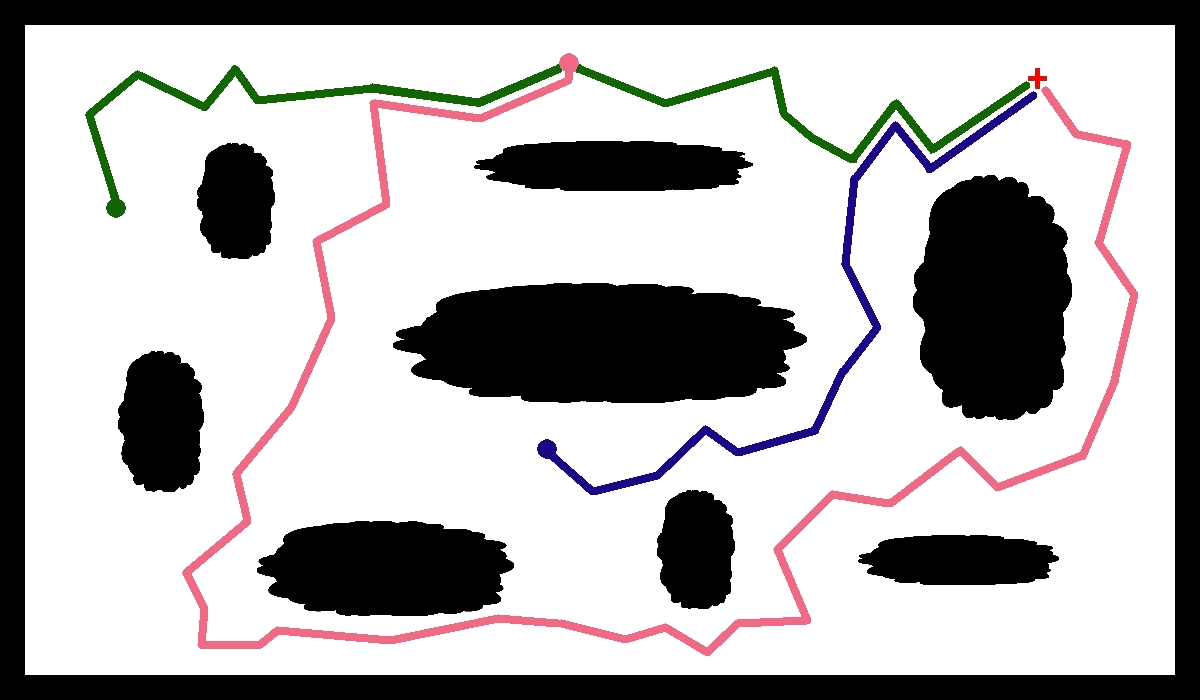
\includegraphics[width=0.7\columnwidth]{figures/instance/Ambush.jpg}}
	
	\vspace{0.15cm}
	\centerline{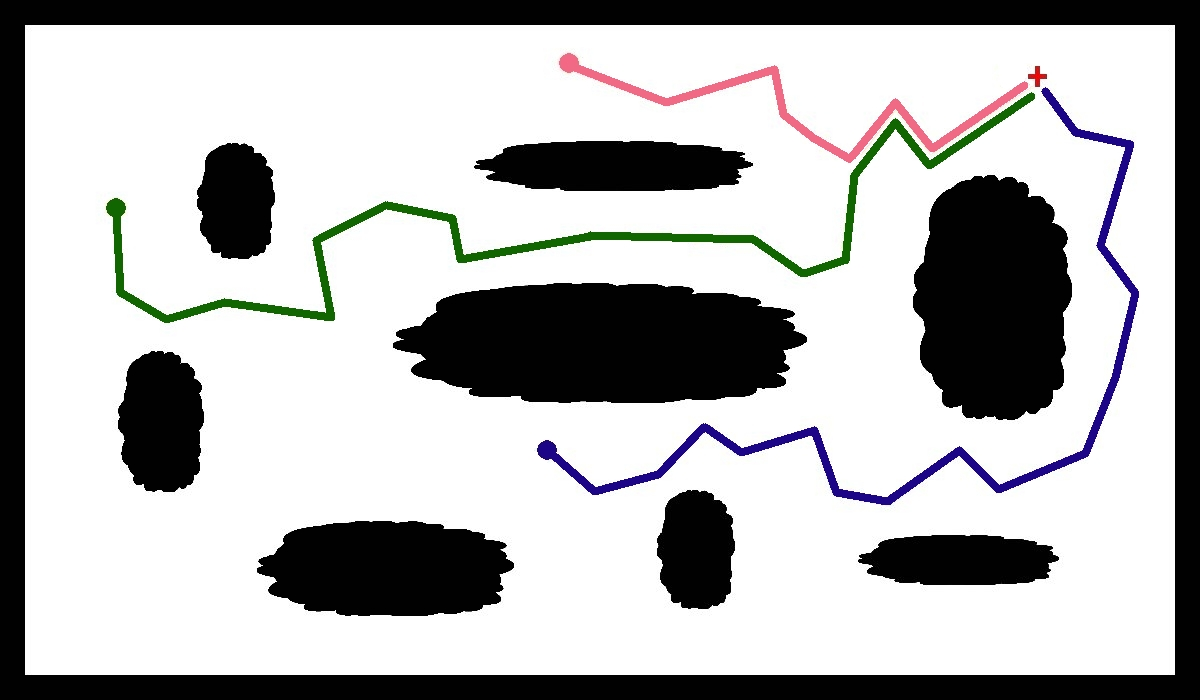
\includegraphics[width=0.7\columnwidth]{figures/instance/Astar-Ambush.jpg}}
	
	\caption{\label{fig:ambush1}
	    Performance of all the algorithms with three agents in map 2. Up: performance of $A^*$. 
	    Middle-Up: Performance of $RST$. Middle-Down: Performance of $A^*mbush$. 
	    Down: performance of $P$-$Ambush$. Both variations of this algorithm gave the 
	    same result for the instance used in the figure.}
\end{figure}


   In the top figure, $A^*$ does not  achieve ambush behavior, 
   $RST$ performs an ambush strategy but
  the random paths the agents take makes the intelligence look poor.
  $A^*mbush$ achieves the desired conduct better than $RST$, but
  the agent that is closest to the goal takes a long and inefficient looking
  path, because it was the last one to calculate it. Both of the $P$-$A^*mbush$
  strategies perform a good ambush without having the problem of
  agents close to the goal taking unintelligent looking paths. This is
  the result of the order in which the elements are performing 
  path calculations. $P$-$A^*mbush$ is letting the agents that
  have the shortest distance to the goal to decide the route first.
  
\begin{table}[h]
\caption{Map1, 5 agents}
\begin{center}

\begin{tabular}{|c|c|c|c|c|c|}
\hline
\# & $A^*$ & $RST$ & $A^*mbush$ & $Euclidean$ & $Real$\\
\hline
f0 & \textbf{1.00} & \textbf{1.00} & \textbf{1.00} & \textbf{1.00} & \textbf{1.00}\\
f1 & 0.67 & 0.67 & \textbf{1.00} & \textbf{1.00} & \textbf{1.00}\\
f2 & \textbf{1.00} & \textbf{1.00} & \textbf{1.00} & \textbf{1.00} & \textbf{1.00}\\
f3 & 0.67 & \textbf{1.00} & \textbf{1.00} & \textbf{1.00} & \textbf{1.00}\\
f4 & \textbf{1.00} & \textbf{1.00} & \textbf{1.00} & \textbf{1.00} & \textbf{1.00}\\
f5 & \textbf{1.00} & \textbf{1.00} & \textbf{1.00} & \textbf{1.00} & \textbf{1.00}\\
f6 & \textbf{1.00} & \textbf{1.00} & \textbf{1.00} & \textbf{1.00} & \textbf{1.00}\\
f7 & \textbf{1.00} & \textbf{1.00} & \textbf{1.00} & \textbf{1.00} & \textbf{1.00}\\
f8 & \textbf{1.00} & \textbf{1.00} & \textbf{1.00} & \textbf{1.00} & \textbf{1.00}\\
f9 & \textbf{1.00} & \textbf{1.00} & \textbf{1.00} & \textbf{1.00} & \textbf{1.00}\\
\hline
n0 & 0.33 & \textbf{0.67} & \textbf{0.67} & \textbf{0.67} & \textbf{0.67}\\
n1 & 0.33 & \textbf{1.00} & \textbf{1.00} & \textbf{1.00} & \textbf{1.00}\\
n2 & 0.50 & \textbf{1.00} & \textbf{1.00} & \textbf{1.00} & \textbf{1.00}\\
n3 & 0.50 & \textbf{1.00} & \textbf{1.00} & \textbf{1.00} & \textbf{1.00}\\
n4 & 0.50 & \textbf{1.00} & \textbf{1.00} & \textbf{1.00} & \textbf{1.00}\\
n5 & 0.33 & \textbf{1.00} & 0.67 & 0.67 & 0.67\\
n6 & 0.33 & \textbf{1.00} & \textbf{1.00} & \textbf{1.00} & \textbf{1.00}\\
n7 & 0.33 & \textbf{1.00} & \textbf{1.00} & \textbf{1.00} & \textbf{1.00}\\
n8 & 0.50 & \textbf{1.00} & \textbf{1.00} & \textbf{1.00} & \textbf{1.00}\\
n9 & 0.33 & 0.67 & \textbf{1.00} & \textbf{1.00} & \textbf{1.00}\\
\hline
\end{tabular}

\label{tab:exp3}
\end{center}
\end{table}


\subsection{Experiments with five agents}
\label{sec:5agents}

Tables \ref{tab:exp3} and \ref{tab:exp4} present
experiments analogous to the ones in section \ref{sec:3agents},
 but using a total of 5 agents.
  
 The overall performance of the proposed ambush
 algorithms becomes better. Except for case n5, the three variations now
 show top values for $\Phi$ every time.  In table \ref{tab:exp3},
  excluding case n4, $A^*mbush$ and $P$-$A^*mbush$ display
 the top value ($\Phi=1$) for the degree of ambush.
 Same goes for table \ref{tab:exp4}, excluding cases n0 and n5.
  This is because  having more agents instantly increases the diversity 
  of the routes. The agents that get to calculate the path last, 
 are not likely to take routes that others are using, since 
 the cost of the common nodes will be significantly bigger.
 
  \begin{table}[h]
\caption{Map 2, 5 agents}
\begin{center}

\begin{tabular}{|c|c|c|c|c|c|}
\hline
\# & $A^*$ & $RST$ & $A^*mbush$ & $Euclidean$ & $Real$\\
\hline
f0 & \textbf{1.00} & \textbf{1.00} & \textbf{1.00} & \textbf{1.00} & \textbf{1.00}\\
f1 & \textbf{1.00} & 0.50 & \textbf{1.00} & \textbf{1.00} & \textbf{1.00}\\
f2 & \textbf{1.00} & \textbf{1.00} & \textbf{1.00} & \textbf{1.00} & \textbf{1.00}\\
f3 & \textbf{1.00} & \textbf{1.00} & \textbf{1.00} & \textbf{1.00} & \textbf{1.00}\\
f4 & \textbf{1.00} & \textbf{1.00} & \textbf{1.00} & \textbf{1.00} & \textbf{1.00}\\
f5 & 0.50 & \textbf{1.00} & \textbf{1.00} & \textbf{1.00} & \textbf{1.00}\\
f6 & \textbf{1.00} & \textbf{1.00} & \textbf{1.00} & \textbf{1.00} & \textbf{1.00}\\
f7 & \textbf{1.00} & \textbf{1.00} & \textbf{1.00} & \textbf{1.00} & \textbf{1.00}\\
f8 & 0.50 & 0.50 & \textbf{1.00} & \textbf{1.00} & \textbf{1.00}\\
f9 & 0.50 & 0.50 & \textbf{1.00} & \textbf{1.00} & \textbf{1.00}\\
\hline
n0 & 0.50 & \textbf{1.00} & \textbf{1.00} & \textbf{1.00} & \textbf{1.00}\\
n1 & 0.33 & 0.67 & \textbf{1.00} & \textbf{1.00} & \textbf{1.00}\\
n2 & 0.50 & \textbf{1.00} & \textbf{1.00} & \textbf{1.00} & \textbf{1.00}\\
n3 & 0.50 & \textbf{1.00} & \textbf{1.00} & \textbf{1.00} & \textbf{1.00}\\
n4 & 0.25 & 0.50 & \textbf{0.75} & \textbf{0.75} & \textbf{0.75}\\
n5 & \textbf{1.00} & 0.50 & \textbf{1.00} & \textbf{1.00} & \textbf{1.00}\\
n6 & 0.33 & 0.67 & \textbf{1.00} & \textbf{1.00} & \textbf{1.00}\\
n7 & 0.33 & 0.67 & \textbf{1.00} & \textbf{1.00} & \textbf{1.00}\\
n8 & 0.50 & \textbf{1.00} & \textbf{1.00} & \textbf{1.00} & \textbf{1.00}\\
n9 & 0.50 & \textbf{1.00} & \textbf{1.00} & \textbf{1.00} & \textbf{1.00}\\
\hline
\end{tabular}

\label{tab:exp4}
\end{center}
\end{table}



\end{comment}

\subsection{Global experiments}
\label{sec:Globals}

The results in this section show the top achieved $\Phi$ value
in bold font. 

\begin{table}[h]
\caption{Ambush rate ($\Phi$) - 2-100 agents}
\begin{center}

\begin{tabular}{|c|c|c|c|c|c||c|c|c|c|c|c|c|}
\hline
 & 
\multicolumn{5}{|c||}{\textbf{Map 1 (60 nodes)}} &
\multicolumn{5}{|c|}{\textbf{Map 2 (85 nodes)}}\\
\hline
\# & $A^*$ & $RST$ & $A^*mbush$ & $P$ & $SAR$ &
	 $A^*$ & $RST$ & $A^*mbush$ & $P$ & $SAR$\\
\hline
 2 & 0.72 & 0.75 & 0.87 & \textbf{0.89} & 0.87 &
	 0.72 & 0.75 & 0.88 & \textbf{0.91} & 0.89\\
 3 & 0.79 & 0.83 & 0.95 & \textbf{0.96} & 0.95 &
	 0.76 & 0.82 & 0.95 & \textbf{0.96} & \textbf{0.96}\\
 4 & 0.85 & 0.90 & 0.98 & \textbf{0.99} & 0.98 &
	 0.83 & 0.88 & 0.98 & \textbf{0.99} & 0.98\\
 5 & 0.89 & 0.93 & \textbf{0.99} & \textbf{0.99} & \textbf{0.99} &
	 0.87 & 0.92 & 0.99 & 0.99 & \textbf{1.00}\\
 6 & 0.91 & 0.96 & \textbf{0.99} & \textbf{0.99} & \textbf{0.99} &
	 0.90 & 0.95 & \textbf{1.00} & 0.99 & \textbf{1.00}\\
 8 & 0.95 & 0.98 & \textbf{0.99} & \textbf{0.99} & \textbf{0.99} &
	0.93 & 0.97 & \textbf{1.00} & \textbf{1.00} & \textbf{1.00}\\
10 & 0.96 & 0.99 & \textbf{1.00} & \textbf{1.00} & \textbf{1.00} &
	 0.95 & 0.99 & \textbf{1.00} & \textbf{1.00} & \textbf{1.00}\\
15 & 0.98 & 0.99 & \textbf{1.00} & \textbf{1.00} & \textbf{1.00} &
	 0.98 & \textbf{1.00} & \textbf{1.00} & \textbf{1.00} & \textbf{1.00}\\
20 & 0.99 & \textbf{1.00} & \textbf{1.00} & \textbf{1.00} & \textbf{1.00} &
     0.99 & \textbf{1.00} & \textbf{1.00} & \textbf{1.00} & \textbf{1.00}\\
50 & 0.99 & \textbf{1.00} & \textbf{1.00} & \textbf{1.00} & \textbf{1.00} &
	\textbf{1.00} & \textbf{1.00} & \textbf{1.00} & \textbf{1.00} & 
	\textbf{1.00}\\
75 & 0.99 & \textbf{1.00} & \textbf{1.00} & \textbf{1.00} & \textbf{1.00} &
	\textbf{1.00} & \textbf{1.00} & \textbf{1.00} & \textbf{1.00} &
	\textbf{1.00}\\
100 & \textbf{1.00} & \textbf{1.00} & \textbf{1.00} & \textbf{1.00} & 
	\textbf{1.00} & 
	\textbf{1.00} & \textbf{1.00} & \textbf{1.00} & \textbf{1.00} & \textbf{1.00}\\
\hline
\end{tabular}

\label{ambushrate}
\end{center}
\end{table}



Tables \ref{ambushrate} and \ref{incr} show global results for
each map, with a variate number of agents. For each case, 1000
random instances of agent's distributions over the polygons
in the map were generated. All the cases are compared by
locating the goal in each node (polygon) of the graph. Finally, 
the mean is taken from this results, and it is shown in the 
tables. 

\begin{comment}
The complete space of possibilities was not explored, given
it's rapid growth. When having $k$ agents in a graph with 
$|V|$ nodes, the total number of possible combinations is
 $|V|^{k+1}$. Each one of this cases must execute the 
 mechanisms proposed for each agent. Having stated this, 
 the total computational complexity would be 
$\bigO( (|V|log|V| + |E|)\cdot k \cdot |V|^{k+1} )$.
\end{comment}

From table \ref{ambushrate} it is noticeable that
when the number of agent increases, the general
$\Phi$ value becomes higher. Also, from more than 8 	
agents, $A^*mbush$, $P$-$A^*mbush$ and 
$SAR$-$A^*mbush$report the maximum $\Phi$.

\begin{table}[h]
\caption{Mean of the Incremental Distance - 2-100 agents}
\begin{center}

\begin{tabular}{|c|c|c|c|c||c|c|c|c|}
\hline
 & 
\multicolumn{4}{|c||}{\textbf{Map 1 (60 nodes)}} &
\multicolumn{4}{|c|}{\textbf{Map 2 (85 nodes)}}\\
\hline
\# & $RST$ & $A^*mbush$ & $P$ & $SAR$ &
	 $RST$ & $A^*mbush$ & $P$ & $SAR$\\
\hline
 2 & 64.54 & 9.00 & 8.54 & \textbf{8.40}   
   & 86.07 & 7.05 & \textbf{6.06} & 7.22\\
 3 & 64.67 & 12.98 & 13.18 & \textbf{9.78}  
   & 84.93 & 12.40 & 11.63 & \textbf{8.91}\\
 4 & 64.99 & 15.13 & 16.54 & \textbf{11.94}
   & 84.24 & 15.50 & 15.97 & \textbf{11.21}\\
 5 & 66.13 & 16.35 & 19.02 & \textbf{12.12}
   & 83.96 & 17.80 & 19.08 & \textbf{11.49}\\
 6 & 64.55 & 16.87 & 20.58 & \textbf{13.01}
   & 85.22 & 18.97 & 21.94 & \textbf{12.56}\\
 8 & 65.53 & 17.62 & 23.94 & \textbf{13.45}
   & 86.81 & 20.89 & 25.96 & \textbf{13.42}\\
10 & 64.93 & 17.45 & 26.21 & \textbf{13.35}
   & 85.88 & 21.42 & 28.86 & \textbf{13.81}\\
15 & 64.24 & 17.51 & 30.15 & \textbf{13.27}
   & 84.91 & 22.15 & 34.43 & \textbf{14.04}\\
20 & 65.22 & 16.88 & 32.11 & \textbf{12.74}
   & 85.22 & 22.00 & 37.22 & \textbf{13.95}\\
50 & 65.13 & 14.19 & 38.42 & \textbf{10.76}
   & 85.06 & 19.02 & 45.00 & \textbf{11.84}\\
75 & 65.03 & 12.86 & 40.42 & \textbf{9.88}
   & 84.77 & 17.48 & 47.31 & \textbf{11.09}\\
100 & 65.27 & 12.08 & 41.88 & \textbf{9.39}
    & 85.26 & 16.47 & 48.88 & \textbf{10.39}\\
\hline
\end{tabular}

\label{incr}
\end{center}
\end{table}



Table \ref{incr} shows the mean of the incremental distance, 
compared against the cost of the path generated by $A^*$ .
This results bring to the light the strong disadvantage
that arises when using $RST$. Since this method only
focuses on generating random routes, it has an mean 
increment of 85.52\% with standard deviation of 0.62 for 
map one, and a mean increment of 64.73\% with standard
deviation of 0.55 for map two. This values don't look
desirable when compared to the ambush family.

Because $A^*mbush$-based methods make the agents take
optimal and and sub-optimal paths, the mean of the incremental
distance is lower. Also, the search performed 
by the ambush based algorithms is informed, so data from the map is 
being used, while with $RST$ only random paths
towards the goal are being pursued. 

$SAR$-$A^*mbush$ shows the lowest increment with a mean of 
11.5\% and 11.66\% for maps one and two respectively,
with standard deviation of 1.78 and 2.1. This result is
expected, since this method makes the agents perform 
$A^*$ for the larger amount of steps possible, while still securing 
 the highest ambush rate that is reachable.  

Results also show that the $P$-$A^*mbush$ technique has
a greater incremental distance than $A^*mbush$ for
maps 1 and 2 specifically, with a mean of 22.35\% and a standard 
deviation 10.40 for map one, while for map two, the mean is 20,98\%
and the standard deviation 7.86.  Nevertheless, section
\ref{sec:Multigraph} will show that this is not true when 
applying the algorithms to graphs with larger number of nodes.
 
Although $P$-$A^*mbush$ increases the cost of the path
of the agents that have less priority, this method increases
the ambush degree, improving the behavior that $A^*mbush$
provided, which is the goal of this research. 

Additionally, both $SAR$-$A^*mbush$ and $P$-$A^*mbush$
 assure a quicker attack and a more intelligent looking behavior.

\subsection{Experiments with multi-scale graphs}
\label{sec:Multigraph}

\begin{table}[h]
\caption{Ambush Rate and Mean of the Incremental Distance 
		 with Multiscale Graphs}
\begin{center}

\begin{tabular}{|c|c|c|c|c|c||c|c|c|c|c|}
\hline
& \multicolumn{5}{|c||}{\textbf{Ambush Rate}} &
  \multicolumn{4}{|c|}{\textbf{Incremental Distance}}\\
\hline
  $Nodes$ & $A^*$ & $RST$ & $A^*mbush$ & $P$ & $SAR$
		  		  & $RST$ & $A^*mbush$ & $P$ & $SAR$\\
\hline
   85 & 0.88 & 0.97 & \textbf{1.00} & \textbf{1.00} & \textbf{1.00}
      & 83.05 & 20.12 & 22.30 & \textbf{13.99}\\
  170 & 0.92 & 0.97 & \textbf{1.00} & 0.99 & \textbf{1.00}
	  & 90.06 & 20.34 & 17.89 & \textbf{12.22}\\
  425 & 0.78 & 0.94 & 0.97 & \textbf{0.98} & \textbf{0.98}
	  & 101.17 & 23.06 & 17.07 & \textbf{11.44}\\
  850 & 0.80 & 0.94 & 0.96 & \textbf{0.97} & \textbf{0.97}
	  & 130.80 & 16.86 & 11.66 & \textbf{6.13}\\
 1700 & 0.76 & 0.94 & \textbf{1.00} & 0.97 & \textbf{1.00}
	  & 119.47 & 9.28 & \textbf{5.35} & 5.96\\
\hline
\end{tabular}

\label{tab:multiscale}
\end{center}
\end{table}


For this experiments, the graphs were automatically generated
 by  concatenations of the map 2 with it's vertical and 
 horizontal flips. Experiments ran under the same conditions 
 than the global experiments, but with a fixed 
number of six agents.

Table \ref{tab:multiscale} shows that the group of $A^*mbush$
based methods have better ambush rates than $A^*$ and $RST$.
They also show smaller increment that the random method.
This means that the desired performance for the proposed
 algorithms does not decrease when the number of 
 nodes increases. In contrast, $A^*$'s ambush
 rates become worse when the size of the graph is bigger.
 
Moreover, table \ref{tab:multiscale} shows that, as the maps
 become larger two important results emerge.
 First, he incremental distance becomes smaller for 
the $A^*mbush$ family. Also, $SAR$-$A^*mbush$ exhibits
better ambush rates than the other ones.
 